% Options for packages loaded elsewhere
\PassOptionsToPackage{unicode}{hyperref}
\PassOptionsToPackage{hyphens}{url}
\PassOptionsToPackage{dvipsnames,svgnames,x11names}{xcolor}
\documentclass[
  10pt,
]{article}
\usepackage{xcolor}
\usepackage[margin=1in]{geometry}
\usepackage{amsmath,amssymb}
\setcounter{secnumdepth}{-\maxdimen} % remove section numbering
\usepackage{iftex}
\ifPDFTeX
  \usepackage[T1]{fontenc}
  \usepackage[utf8]{inputenc}
  \usepackage{textcomp} % provide euro and other symbols
\else % if luatex or xetex
  \usepackage{unicode-math} % this also loads fontspec
  \defaultfontfeatures{Scale=MatchLowercase}
  \defaultfontfeatures[\rmfamily]{Ligatures=TeX,Scale=1}
\fi
\usepackage{lmodern}
\ifPDFTeX\else
  % xetex/luatex font selection
\fi
% Use upquote if available, for straight quotes in verbatim environments
\IfFileExists{upquote.sty}{\usepackage{upquote}}{}
\IfFileExists{microtype.sty}{% use microtype if available
  \usepackage[]{microtype}
  \UseMicrotypeSet[protrusion]{basicmath} % disable protrusion for tt fonts
}{}
\makeatletter
\@ifundefined{KOMAClassName}{% if non-KOMA class
  \IfFileExists{parskip.sty}{%
    \usepackage{parskip}
  }{% else
    \setlength{\parindent}{0pt}
    \setlength{\parskip}{6pt plus 2pt minus 1pt}}
}{% if KOMA class
  \KOMAoptions{parskip=half}}
\makeatother
\usepackage{longtable,booktabs,array}
\usepackage{caption}
\captionsetup[table]{skip=6pt}
\newcounter{none} % for unnumbered tables
\usepackage{calc} % for calculating minipage widths
% Correct order of tables after \paragraph or \subparagraph
\usepackage{etoolbox}
\makeatletter
\patchcmd\longtable{\par}{\if@noskipsec\mbox{}\fi\par}{}{}
\makeatother
% Allow footnotes in longtable head/foot
\IfFileExists{footnotehyper.sty}{\usepackage{footnotehyper}}{\usepackage{footnote}}
\makesavenoteenv{longtable}
\usepackage{graphicx}
\makeatletter
\newsavebox\pandoc@box
\newcommand*\pandocbounded[1]{% scales image to fit in text height/width
  \sbox\pandoc@box{#1}%
  \Gscale@div\@tempa{\textheight}{\dimexpr\ht\pandoc@box+\dp\pandoc@box\relax}%
  \Gscale@div\@tempb{\linewidth}{\wd\pandoc@box}%
  \ifdim\@tempb\p@<\@tempa\p@\let\@tempa\@tempb\fi% select the smaller of both
  \ifdim\@tempa\p@<\p@\scalebox{\@tempa}{\usebox\pandoc@box}%
  \else\usebox{\pandoc@box}%
  \fi%
}
% Set default figure placement to htbp
\def\fps@figure{htbp}
\makeatother
\setlength{\emergencystretch}{3em} % prevent overfull lines
\providecommand{\tightlist}{%
  \setlength{\itemsep}{0pt}\setlength{\parskip}{0pt}}
\usepackage{bookmark}
\IfFileExists{xurl.sty}{\usepackage{xurl}}{} % add URL line breaks if available
\urlstyle{same}
% fallback for those not using the hyperref driver hyperxmp:
\makeatletter
\@ifundefined{xmpquote}{\newcommand{\xmpquote}[1]{#1}}{}
\makeatother
\hypersetup{
  colorlinks=true,
  linkcolor={Maroon},
  filecolor={Maroon},
  citecolor={Blue},
  urlcolor={Blue},
  pdfcreator={LaTeX via pandoc}}

\title{CS683 PA1: Task2}
\author{\textbf{Team: Huffman} \\[3pt]
  Shaik Awez Mehtab (23b1080), Satyam Sinoliya (23b0958), \\
  Gautam Siddarth (23b0957), Mohana Evuri (23b1017)}
\date{}

\begin{document}
\maketitle
\section{Task 2: Matrix Multiplication}\label{task-2-matmul}

\subsection{Setup}\label{setup2}

\begin{itemize}
\tightlist
\item
  Intel Core i5-12450H (4 P-cores + 4 E-cores). L1d 48 KiB/core, L2 1.25
  MiB/P-core, L3 12 MiB shared.
\item
  Hardware prefetchers \textbf{disabled}, except in experiment F, which
  measures both states because that is what 2A.5 asks for.
\item
  Everything pinned with \texttt{taskset\ -c\ 2}, so the process cannot
  migrate between a P-core and an E-core mid-run.
\item
  \texttt{./bin/matmul} is the given harness, used for the graded result.
\item
  \texttt{perf\_bench/} runs a single stage with no correctness pass, so
  \texttt{perf} counters belong to that kernel alone. The graded harness always
  runs naive too, which would swamp the counters. All tables here come from it.
\item
  \texttt{scripts/} has one script per experiment, each writing a CSV into
  \texttt{results/}. \texttt{plot\_all.py} turns those into the figures.
\item
  \texttt{simd\_width\_bench/} holds the 128-bit and 512-bit variants for 2B,
  since the given tree has no file for them.
\item
  The counters are named by what we want, and resolved to whatever this CPU
  calls them:
\end{itemize}

{\def\LTcaptype{none} % do not increment counter
\begin{longtable}[]{@{}ll@{}}
\toprule\noalign{}
what we wanted & event used \\
\midrule\noalign{}
\endhead
\bottomrule\noalign{}
\endlastfoot
L1-D misses & \texttt{MEM\_LOAD\_RETIRED.L1\_MISS} \\
L1-D accesses & \texttt{MEM\_INST\_RETIRED.ALL\_LOADS} \\
L2 misses & \texttt{l2\_rqsts.miss} \\
LLC misses & \texttt{LONGEST\_LAT\_CACHE.MISS} \\
software prefetches & \texttt{sw\_prefetch\_access.any} \\
\end{longtable}
}

\begin{itemize}
\tightlist
\item
  The governor is set to \texttt{performance}. On \texttt{powersave} the clock
  ramps mid-run and the wall clock becomes unusable, which we ran into and
  describe in 2A.3. Experiment C was taken before we fixed the governor, but it
  only reports miss counts and IPC, which do not depend on the clock.
\end{itemize}
\subsection{What each stage does}\label{stages2}

\begin{itemize}
\item
  \texttt{matmul\_naive} is the given triple loop. \texttt{B} is indexed as
  \texttt{B[j * ldb + p]}, so it is already stored transposed and both operands
  are read contiguously. There is no stride problem to fix here, which is why
  the wins in this task come from vectorising and from keeping the operands in
  cache, not from reordering loops.

\item
  \texttt{matmul\_simd} keeps the same loop nest and vectorises the dot product
  with 256-bit FMAs. It runs \textbf{four independent accumulators}, folds them
  at the end, and finishes the leftover elements with one vector and then
  scalars. The four accumulators matter because a single one would make every
  FMA wait on the previous one.

\item
  \texttt{matmul\_prefetch} blocks the loops over M, N and K, and issues
  \texttt{\_mm\_prefetch} for \texttt{A} and \texttt{B} one cache line at a time,
  \texttt{PREFETCH\_DIST} floats ahead. It stays scalar on purpose, so 2A
  measures prefetching and not vectorisation. Blocking over K means each dot
  product is split into partial sums, so \texttt{C} has to be zeroed first and
  accumulated across K-blocks.

\item
  \texttt{matmul\_optimized} combines both and adds a register tile: a 4x3 block
  of \texttt{C} held in 12 vector accumulators, which is 12 FMAs for every 7
  vector loads. A 4x4 tile would need 24 live vectors and spill, so 4x3 is the
  largest that fits the 16 YMM registers. It also batches the horizontal sums
  four at a time, and keeps a 1x4 fallback for leftover rows.
\end{itemize}

\subsection{Task 2A: Software prefetching}\label{task-2a}

\subsubsection{1. Impact of the matrix size}\label{a-size}

Times in ms, best of 3, all four stages at each size:

{\def\LTcaptype{none} % do not increment counter
\begin{longtable}[]{@{}llllll@{}}
\toprule\noalign{}
size & naive & simd & prefetch & optimized & optimized speedup \\
\midrule\noalign{}
\endhead
\bottomrule\noalign{}
\endlastfoot
128 & 0.71 & 0.07 & 0.70 & 0.05 & 15.23x \\
256 & 6.66 & 0.61 & 6.62 & 0.36 & 18.50x \\
512 & 63.02 & 7.24 & 61.07 & 3.85 & 16.35x \\
1024 & 536.64 & 87.17 & 498.73 & 34.21 & 15.69x \\
2048 & 4995.17 & 1180.52 & 4165.35 & 287.37 & 17.38x \\
\end{longtable}
}

\begin{itemize}
\item
  \texttt{prefetch} climbs steadily with size: 1.02x, 1.01x, 1.03x, 1.08x,
  \textbf{1.20x}. At 128 the whole problem is 192 KiB and already sits in cache,
  so there is nothing to prefetch and we only pay for the extra instructions.

\item
  The gain grows with size, which is what we expected: prefetching can only help
  once the operands stop fitting in cache and the loads actually have to wait.

\item
  \texttt{simd} peaks at 256 and then falls off (10.94x to 4.23x). It has no
  blocking at all, so once the matrices leave cache it becomes memory bound and
  the extra FMA throughput has nowhere to go.

\item
  \texttt{optimized} holds 15-18x across the whole range, because it is the only
  stage that blocks for cache and vectorises at the same time.
\end{itemize}

\begin{figure}
\centering
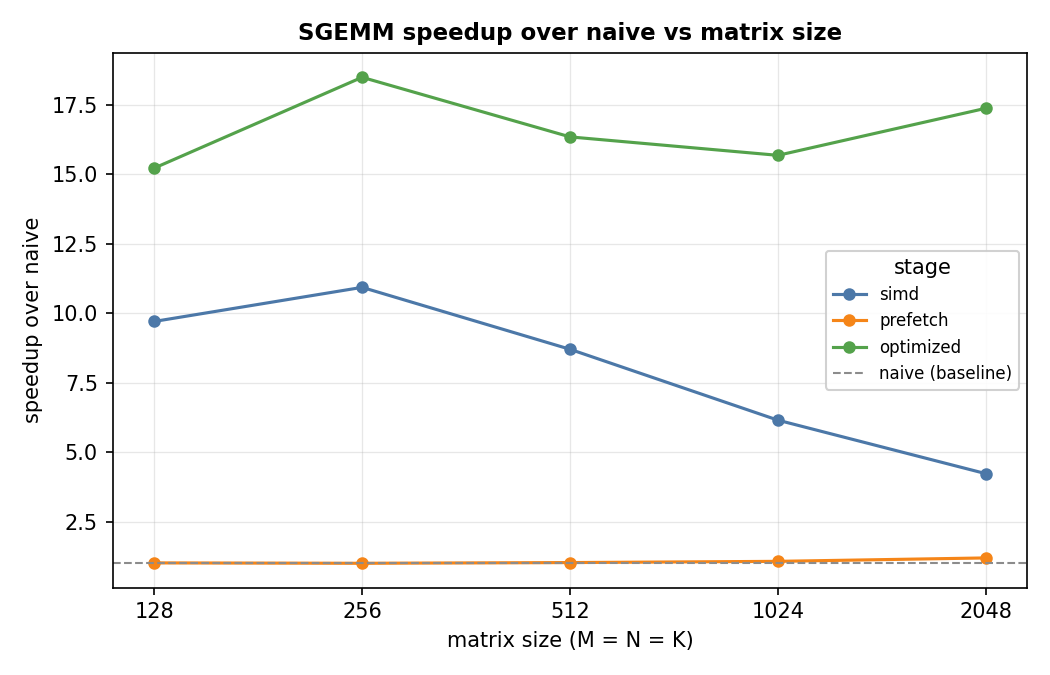
\includegraphics[width=0.88\linewidth,height=\textheight,keepaspectratio,alt={Speedup over naive vs matrix size for each stage.}]{../plots/task2_speedup_vs_size.png}
\caption{Speedup over naive vs matrix size, all stages.}
\end{figure}

\subsubsection{2. CPU metrics}\label{a-metrics}

At 1024, from \texttt{perf}, counted on the kernel alone:

{\def\LTcaptype{none} % do not increment counter
\begin{longtable}[]{@{}lllll@{}}
\toprule\noalign{}
stage & L1-D MPKI & L2 misses & LLC misses & IPC \\
\midrule\noalign{}
\endhead
\bottomrule\noalign{}
\endlastfoot
naive & 10.18 & 269.2 M & 3.43 M & 3.07 \\
simd & 152.64 & 269.0 M & 0.75 M & 1.52 \\
prefetch & 9.02 & 11.6 M & 4.75 M & 3.77 \\
optimized & 43.61 & 3.3 M & 0.71 M & 3.94 \\
\end{longtable}
}

\begin{itemize}
\item
  The number that matters is \textbf{L2 misses}: blocking plus prefetching takes
  it from 269 M down to 11.6 M, a \textbf{23x} cut, and \texttt{optimized} gets
  it to 3.3 M. That is the whole point of 2A and it is invisible in the timing
  table, because the scalar loop is slow for other reasons.

\item
  \texttt{simd} has the same 269 M L2 misses as naive. It never touches the
  memory side, it only makes the compute part faster, so at 1024 it is left
  waiting on exactly the same traffic.

\item
  \texttt{simd}'s L1 MPKI of 152 looks alarming but is an artefact of the metric:
  it executes 9x fewer instructions than naive for the same misses, so the
  denominator collapses. Its absolute L1 miss count is the same as naive's.
\end{itemize}

\begin{figure}
\centering
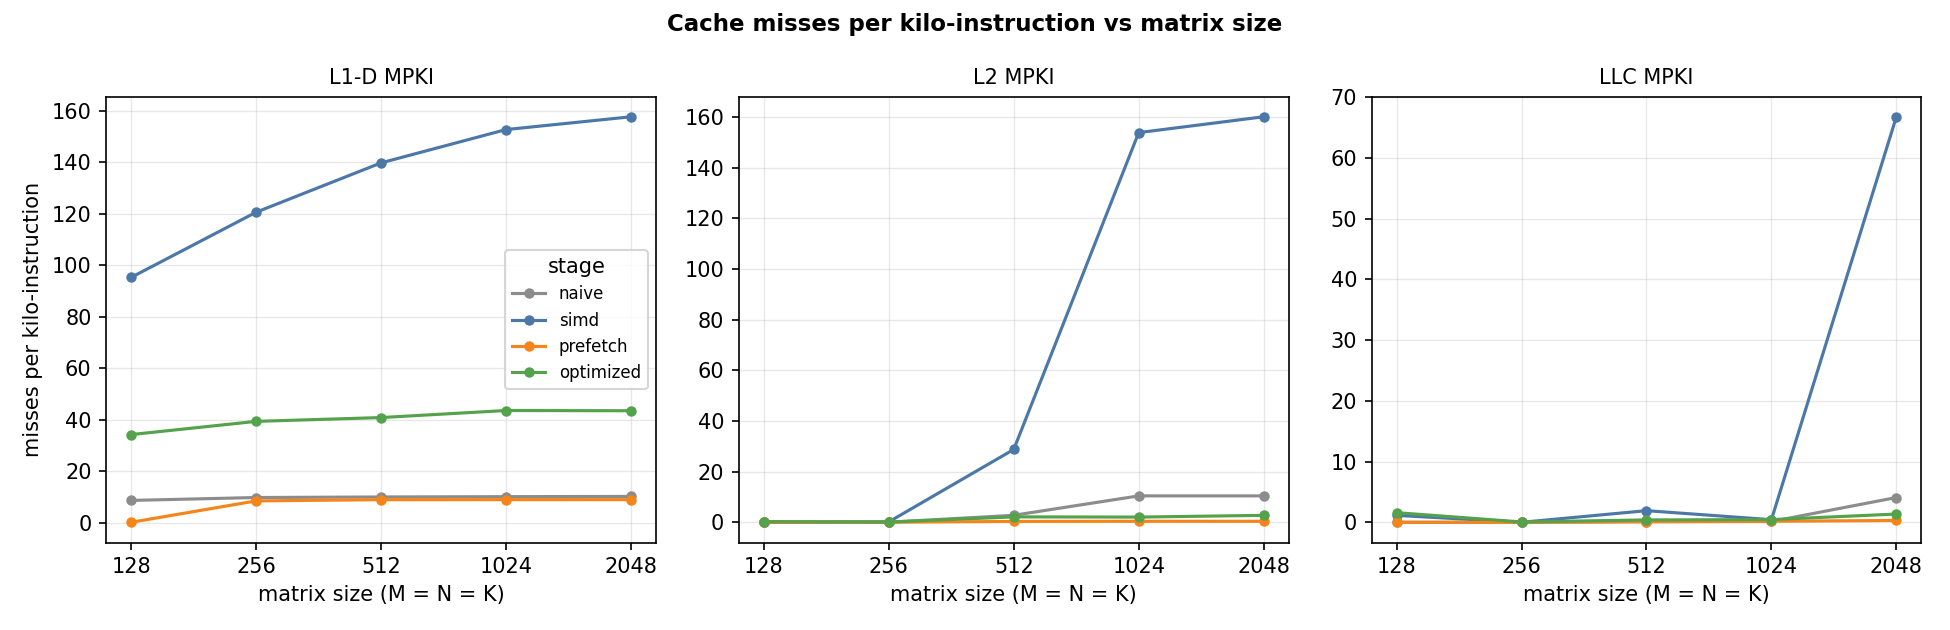
\includegraphics[width=0.88\linewidth,height=\textheight,keepaspectratio,alt={L1-D, L2 and LLC MPKI vs matrix size for each stage.}]{../plots/task2_mpki_vs_size.png}
\caption{Cache metrics vs matrix size.}
\end{figure}

\subsubsection{3. Execution time and speedup}\label{a-speedup}

\begin{itemize}
\item
  2A defines speedup as time \emph{without} software prefetching over time
  \emph{with} it, so the baseline has to be the same kernel with the prefetches
  removed. \texttt{PREFETCH\_DIST=0} compiles every \texttt{\_mm\_prefetch} away,
  and the scripts check the disassembly to confirm the baseline really contains
  zero prefetch instructions before using it.

\item
  We report this speedup in \textbf{cycles, not wall time}. These runs were made
  before we switched the governor to \texttt{performance}, and
  \texttt{powersave} distorted the wall clock badly: the no-prefetch baseline at
  1024 took 879 ms but only 7.694 Gcycles, while the dist=64 build took 462 ms at
  7.440 Gcycles. Nearly the same work in half the time, because the baseline ran
  at roughly half clock. By wall time that reads as 1.90x, which is not real.
  Cycles do not have that problem.
\end{itemize}

\subsubsection{4. Optimal prefetch distance and cache fill
level}\label{a-optimal}

\texttt{prefetch} at 1024, baseline 7.694 Gcycles:

{\def\LTcaptype{none} % do not increment counter
\begin{longtable}[]{@{}llll@{}}
\toprule\noalign{}
distance (floats) & bytes & Gcycles & speedup \\
\midrule\noalign{}
\endhead
\bottomrule\noalign{}
\endlastfoot
8 & 32 & 7.671 & 1.003x \\
16 & 64 & 8.469 & 0.909x \\
\textbf{32} & \textbf{128} & \textbf{7.440} & \textbf{1.034x} \\
\textbf{64} & \textbf{256} & \textbf{7.440} & \textbf{1.034x} \\
128 & 512 & 7.450 & 1.033x \\
256 & 1024 & 7.455 & 1.032x \\
512 & 2048 & 7.452 & 1.033x \\
\end{longtable}
}

\begin{itemize}
\item
  Anything from 32 floats onwards gives the same \textasciitilde1.03x, so the
  curve is flat rather than peaked. 8 is too short to cover the miss latency, and
  past 32 the prefetch has already landed by the time we need it.

\item
  Fill level, same stage and size, distance fixed at 64: T0 1.043x, T1 1.052x,
  T2 1.044x, NTA 1.050x. \textbf{T1 is best}, but the whole spread is 1\%. We
  measured this twice, before and after fixing the CPU governor, and the
  ordering changed between the two runs, so the fill level does not really
  matter for this kernel.
\end{itemize}

\begin{figure}
\centering
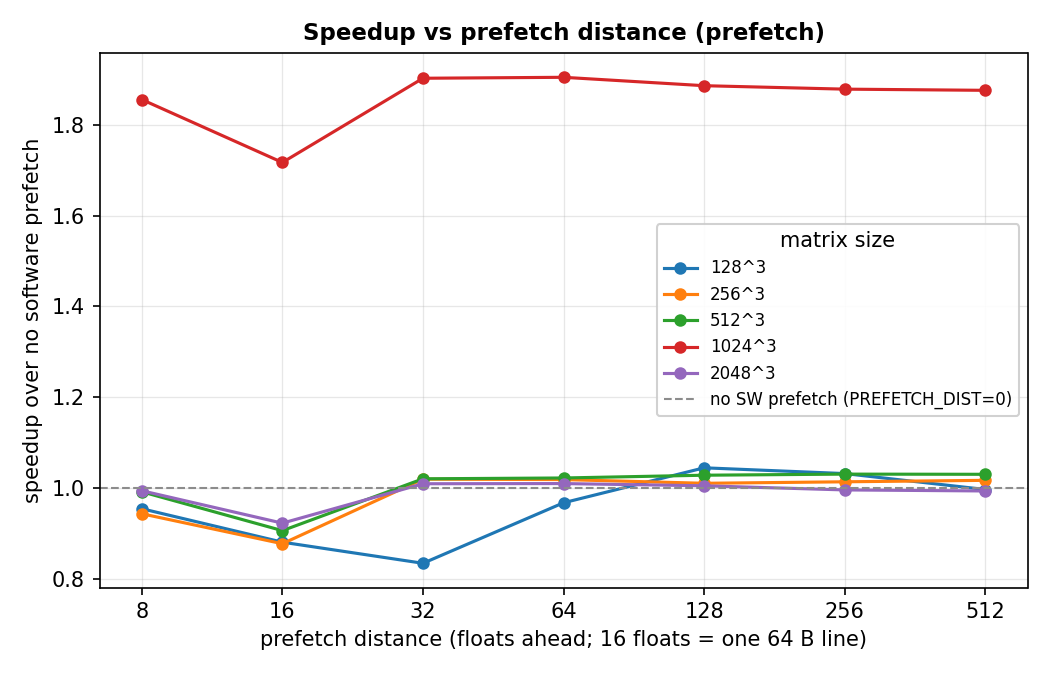
\includegraphics[width=0.88\linewidth,height=\textheight,keepaspectratio,alt={Speedup vs prefetch distance.}]{../plots/task2_prefetch_degree.png}
\caption{Speedup vs prefetch distance.}
\end{figure}

\begin{figure}
\centering
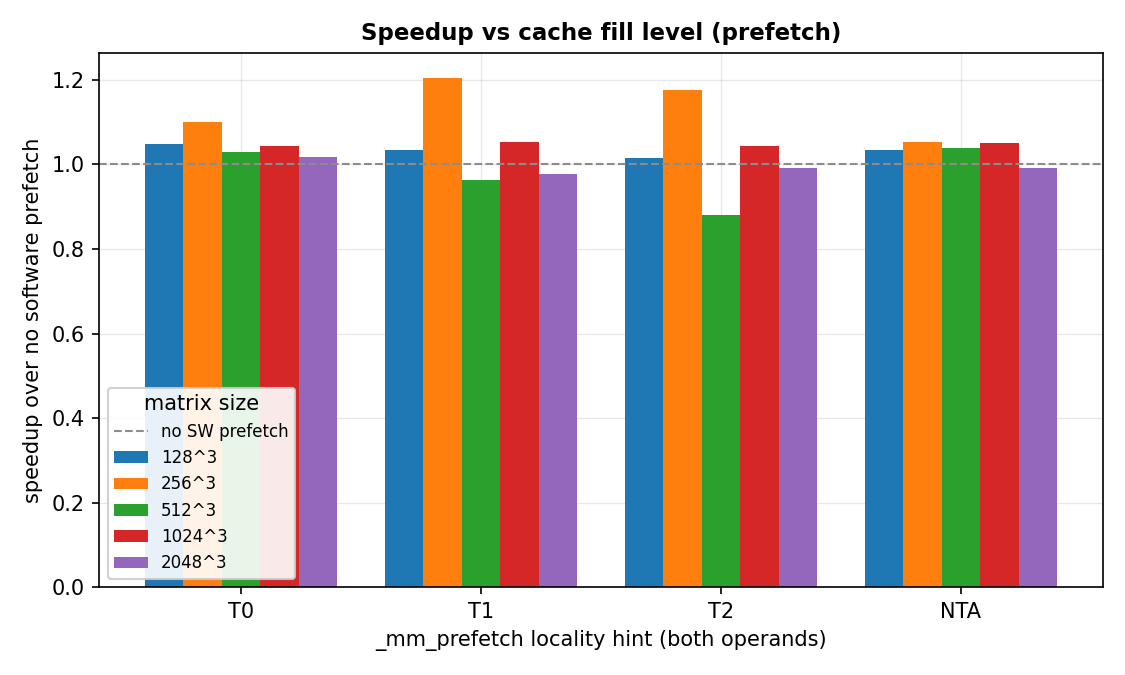
\includegraphics[width=0.88\linewidth,height=\textheight,keepaspectratio,alt={Speedup vs cache fill level hint.}]{../plots/task2_prefetch_level.png}
\caption{Speedup vs cache fill level (T0 / T1 / T2 / NTA).}
\end{figure}

\subsubsection{5. Effect of the hardware
prefetchers}\label{a-hwpf}

We toggled all four prefetchers through MSR \texttt{0x1A4} (0x0 = on, 0xF =
off) and measured each stage in both states, software prefetch left on:

{\def\LTcaptype{none} % do not increment counter
\begin{longtable}[]{@{}lllllll@{}}
\toprule\noalign{}
stage & size & time on & time off & L1D MPKI on & L1D MPKI off & miss ratio \\
\midrule\noalign{}
\endhead
\bottomrule\noalign{}
\endlastfoot
simd & 1024 & 76.1 & 87.1 & 139.09 & 152.37 & 1.10x \\
simd & 2048 & 1111.6 & 1095.9 & 131.49 & 156.34 & 1.19x \\
prefetch & 1024 & 510.3 & 501.4 & 1.43 & 9.03 & \textbf{6.29x} \\
prefetch & 2048 & 4266.0 & 4019.4 & 1.32 & 9.03 & \textbf{6.83x} \\
optimized & 1024 & 35.6 & 36.7 & 26.18 & 43.48 & 1.66x \\
optimized & 2048 & 285.0 & 290.5 & 26.09 & 43.48 & 1.67x \\
\end{longtable}
}

\begin{itemize}
\item
  The prefetchers do what they are supposed to: turning them off multiplies L1
  misses by \textbf{6.3x} on the blocked scalar kernel and 1.67x on
  \texttt{optimized}. The effect is real and large.

\item
  But the \textbf{time barely moves}, between 0.94x and 1.15x either way. So
  those misses were not what the kernel was waiting on. Only \texttt{simd} at
  1024 shows a real gain (15\%), and that is the one stage with no blocking, so
  it is the only one actually stalling on memory.

\item
  Software prefetching matters more when the hardware ones are off, which is
  what we would expect since they are doing the same job. On \texttt{prefetch}
  at 1024 it is worth 1.127x with the hardware prefetchers off but only 1.023x
  with them on.

\item
  This CPU has no hardware-prefetch event we could count, so the
  \texttt{hwpf\ events} column reads 0 throughout and the toggle cannot be
  confirmed from a counter directly. The 6.3x jump in L1 misses is the evidence
  that the MSR write landed.
\end{itemize}

\begin{figure}
\centering
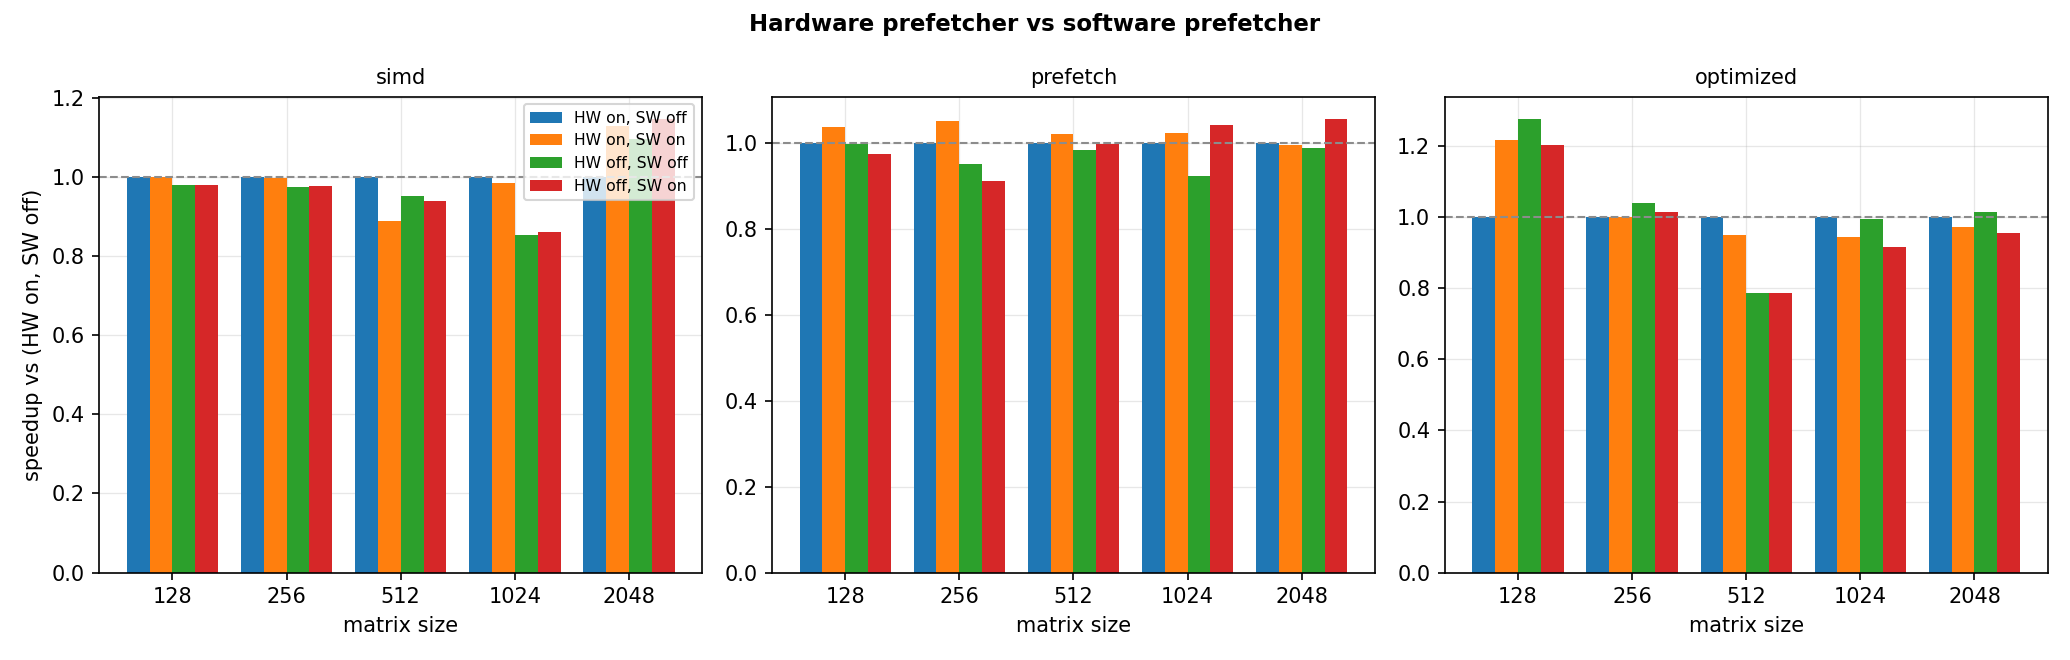
\includegraphics[width=0.88\linewidth,height=\textheight,keepaspectratio,alt={Time and L1-D MPKI with hardware prefetchers on versus off.}]{../plots/task2_hw_prefetcher.png}
\caption{Hardware prefetchers on vs off, per stage and size.}
\end{figure}

\subsubsection{Answers}\label{a-answers}

\begin{itemize}
\item
  \textbf{Q1. Trend in speedup with matrix size.} It grows with size, from 1.02x
  at 128 to 1.20x at 2048. Small matrices already fit in cache, so the prefetches
  only add instructions and buy nothing. The bigger the matrix, the more real
  misses there are for a prefetch to hide.

\item
  \textbf{Q2. Best prefetch distance.} \textbf{32 to 64 floats} (128-256 bytes),
  worth 1.03x. Everything from 32 up is within noise of each other.

\item
  \textbf{Q3. Best cache fill level.} \textbf{T1}, at 1.052x, but T0/T2/NTA are
  all within 1\% of it, and a repeat run reordered them, so the choice does not
  really matter for this kernel.
\end{itemize}

\subsection{Task 2B: SIMD}\label{task-2b}

\begin{itemize}
\item
  \texttt{simd\_width\_bench/} holds a 128-bit (SSE), a 256-bit (AVX2) and a
  512-bit (AVX-512) variant of the same dot product, so only the vector width
  changes between them.

\item
  \textbf{AVX-512 is not available on this CPU}, so the 512-bit variant is
  compiled but reported as unsupported rather than measured. Only 128 and 256
  bit are in the tables.
\end{itemize}

Instructions per run and time, at each size (Table 2.1 form):

{\def\LTcaptype{none} % do not increment counter
\begin{longtable}[]{@{}llllll@{}}
\toprule\noalign{}
size & metric & no SIMD & 128-bit & 256-bit & 512-bit \\
\midrule\noalign{}
\endhead
\bottomrule\noalign{}
\endlastfoot
512 & instructions & 8.08e8 & 2.07e8 & 8.91e7 & n/a \\
512 & time (ms) & 71.74 & 17.33 & 10.48 & n/a \\
512 & speedup & 1.00x & 4.14x & 6.85x & n/a \\
1024 & instructions & 6.45e9 & 1.62e9 & 6.92e8 & n/a \\
1024 & time (ms) & 554.52 & 155.68 & 110.40 & n/a \\
1024 & speedup & 1.00x & 3.56x & 5.02x & n/a \\
2048 & instructions & 5.16e10 & 1.29e10 & 5.45e9 & n/a \\
2048 & time (ms) & 5170.66 & 2054.72 & 1398.19 & n/a \\
2048 & speedup & 1.00x & 2.52x & 3.70x & n/a \\
\end{longtable}
}

\begin{itemize}
\item
  Instructions drop by \textbf{3.9x} at 128-bit and \textbf{9.3x} at 256-bit,
  and those factors are the same at every size. That is close to the 4 and 8
  lanes the two widths give us, with the extra coming from the loop running 4 or
  8 times fewer iterations, so the loads, increments and branches divide too.

\item
  Speedup is nowhere near the instruction reduction: 9.3x fewer instructions
  buys only 5.0x at 1024 and 3.7x at 2048. The kernel is not vectorised into
  being compute bound, it just reaches the memory wall sooner.

\item
  This is the same effect as in Task 1C. The wider version removes more
  instructions, so it hits the point where it is waiting on memory earlier, and
  past that width stops paying.
\end{itemize}

\begin{figure}
\centering
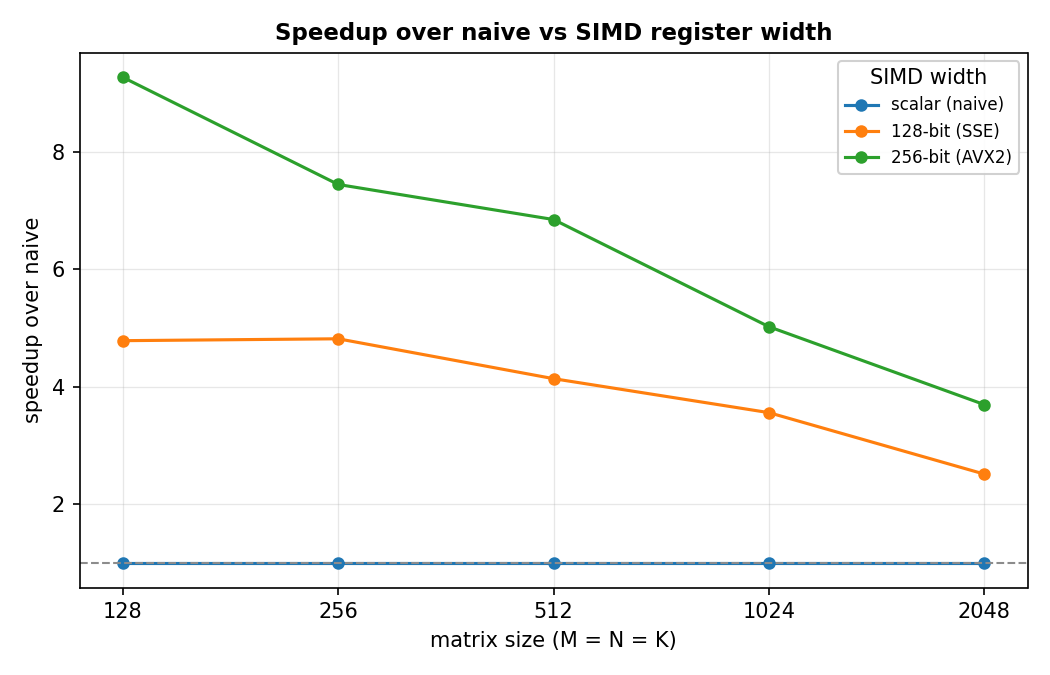
\includegraphics[width=0.88\linewidth,height=\textheight,keepaspectratio,alt={Speedup vs matrix size for 128-bit and 256-bit SIMD.}]{../plots/task2_simd_width_speedup.png}
\caption{Speedup by SIMD width vs matrix size.}
\end{figure}

\begin{figure}
\centering
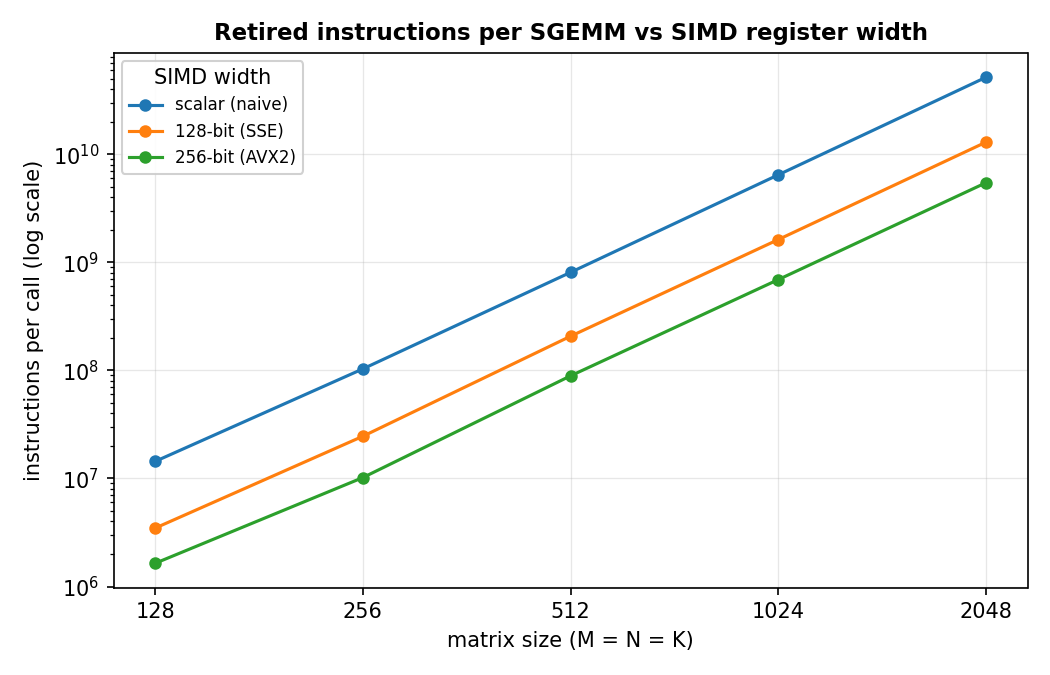
\includegraphics[width=0.88\linewidth,height=\textheight,keepaspectratio,alt={Instruction count by SIMD width.}]{../plots/task2_simd_width_instructions.png}
\caption{Instructions per run by SIMD width.}
\end{figure}

\subsubsection{Answers}\label{b-answers}

\begin{itemize}
\item
  \textbf{Q1. Trends across sizes and widths.} Wider is always faster, but the
  advantage shrinks as the matrix grows: 256-bit over 128-bit is 1.65x at 512,
  1.41x at 1024 and 1.47x at 2048, while both fall steeply in absolute terms
  (6.85x to 3.70x for 256-bit). The instruction saving is constant with size,
  so everything we lose at large sizes is memory, not compute.

\item
  \textbf{Q2. Which width gives the maximum speedup.} \textbf{256-bit (AVX2)},
  at 6.85x at 512. AVX-512 would presumably go further but this CPU does not
  have it.
\end{itemize}

\subsection{Task 2C: Software prefetching + SIMD}\label{task-2c}

\texttt{matmul\_optimized} is the combination: register tiling, cache blocking
over M/N/K, 256-bit FMAs and software prefetch together.

{\def\LTcaptype{none} % do not increment counter
\begin{longtable}[]{@{}lllll@{}}
\toprule\noalign{}
size & SIMD only & prefetch only & both & L2 misses (both) \\
\midrule\noalign{}
\endhead
\bottomrule\noalign{}
\endlastfoot
256 & 10.94x & 1.01x & 18.50x & \\
512 & 8.71x & 1.03x & 16.35x & \\
1024 & 6.16x & 1.08x & 15.69x & 3.3 M \\
2048 & 4.23x & 1.20x & 17.38x & 35.3 M \\
\end{longtable}
}

\begin{itemize}
\item
  The two compose well: at 1024, SIMD alone gives 6.16x and prefetching alone
  1.08x, which multiplied would be 6.6x, but together we get \textbf{15.7x}.

\item
  The reason is the same as in Task 1D. Each one removes the limit that was
  hiding the other. SIMD alone stays stuck on memory traffic (269 M L2 misses,
  same as naive). Blocking alone fixes the traffic but leaves the loop scalar.
  Only with both is it neither.

\item
  \textbf{Software prefetching is the smallest part of this.} Measured on
  \texttt{optimized} alone at 1024, turning the prefetches on gives
  \textbf{0.96x}, so it slightly hurts. Instructions go from 1.27e9 to 1.60e9,
  a 26\% increase, while L1 misses barely move (74.1 M to 69.7 M).

\item
  That makes sense: once the kernel is register tiled and cache blocked, the
  operands are already close by, so there is not much latency left for a
  prefetch to hide, and we just pay for the extra instructions. Prefetching
  pays off on the scalar blocked kernel (1.03x) and not on the tuned one.
\end{itemize}

\subsection{Final results}\label{final2}

Graded harness (\texttt{./bin/matmul}, M=N=K=1024, seed 1234):

\begin{verbatim}
correctness : 30 / 30   (3 of 3 stages correct)
optimized   : 18.20x  ->  55 / 70  speedup points
TOTAL       :  85 / 100
\end{verbatim}

\begin{itemize}
\item
  The reported speedup is \textbf{noisy}: three consecutive runs on an idle
  machine with the performance governor gave 11.51x, 14.19x and 18.20x. The
  scoring tier changes at 18x, so the same binary scores either 70 or 85 out of
  100 depending on the run.

\item
  The same source on a teammate's machine (Core 7 150U, 5.4 GHz, 6.5 MiB L2)
  reaches 23.5x at 1024 and 25.3x at 2048. The kernel moves about 1.2 bytes per
  flop, so it is bound by L2 capacity and clock, which is exactly where the two
  CPUs differ. Nothing in the source changed between those two numbers.

\item
  All three stages were checked against the naive reference by the harness at
  every size we measured, and separately at 257 (a non-multiple of the block and
  vector sizes) by the experiment scripts.
\end{itemize}

\end{document}
